\chapter{IDEA testbeams}
\label{chapter:ideatestbeam}

\epigraph{[new quote split \\ over two lines]}{[author]}

While \acrshort{DQM4hep} was intended from the beginning as a generic tool, it was developed largely within the AIDA-2020 collaboration, which also promoted a variety of standards and guidelines for data acquisition devices, data formats, etc. In addition to this, it was also only tested on calorimeter-type detectors within the \acrshort{CALICE} collaboration. To be sure that \acrshort{DQM4hep} was truly generic -- capable of adapting to \textit{any} detector -- it was necessary to test it on a wider variety of detectors outside of the AIDA-2020 and \acrshort{CALICE} collaborations.

An ideal opportunity arose for this in the form of the \acrshort{IDEA} testbeam. This testbeam was run by a collaboration of Italian and American universities working on four different particle physics detectors of different types, intending to run a single combined testbeam of all four instruments at the \acrshort{CERN} \acrshort{SPS} in September 2018. \acrshort{DQM4hep} was offered as a possible unified monitoring solution that could integrate information from all four detectors into the same tool. This provided convenience for the teams operating the testbeam and detectors, and an extremely valuable opportunity to test \acrshort{DQM4hep} out of its established operating range.

\section{Introduction}
The combined testbeam took place between in September 2018 at the \acrshort{CERN} \acrshort{SPS} beamline facility. The testbeam itself lasted a week, from the 5th-12th September, with a preparation period of one week before this for installation, calibration, etc. [...]

\subsection*{Detectors at the combined testbeam}
The combined testbeam comprised four separate dectors: a calorimeter, a muon detector and preshower, a drift chamber, and a silicon photomultiplier. One of the biggest challenges involved in the testbeam was operating these four different detectors [...]

\subsubsection{RD52 calorimeter} % Another reference: https://arxiv.org/pdf/1703.09120.pdf
The \acrfull{DREAM} calorimeter, also called the RD52 calorimeter, is a dual-readout calorimeter built, developed and tested by the RD52 collaboration by researchers based in universities at Gagliari, Cosenza, Pavia, Pisa, Rome, Iowa State and Texas Tech. 

The aim of the calorimeter is to use both the \v{C}erenkov and scintillator techniques simultaneously (hence ``dual-readout'') to improve calorimetry, especially using calorimeters to measure four-vectors of jets and single hadrons, which suffer a reduced precision compared to electrons and photons. By comparing signals from \v{C}erenkov light and scintillator light, the electromagnetic shower fraction can be measured on an event-by-event basis, eliminating the effects of fluctuations. %Reference here: https://iopscience.iop.org/article/10.1088/1742-6596/404/1/012068/pdf

%-Nine lead modules (9.3x9.3x150cm^3)
%-Sampling fraction 5%, PMT readout
%-Hadronic energy resolution in 4pi geometry should be 30%/sqrt(E)

\subsubsection{Muon chamber and preshower}
[...]

%Muon chamber
%-One triple-GEM, same as preshower
%-Two micro-RWELL 10x10cm^2 (40 micron spatial resolution, rates up to 10MHz/cmm^2)

%Preshower
%-Lead absorber with fixed 5mm layer, but can vary from 1 to 2.5 X_0
%-Two triple-GEM detectors
%-10x10cm^2 surface area, strip readout, 650 micron pitch
%-Ar/CO2/CF4 gas used for testbeam
%-Efficiency 97% based on previous testbeams
%-Spatial resolution 100 microns

\subsubsection{Silicon photomultiplier GEM}
[...]

\subsubsection{Drift chamber}
[...]

%-12 layers, with 12 1x1cm^2 drift cells per layer
%-144 channels total
%-resolution is 100 micron in x-y, 1mm in z

\subsubsection{Ancillary detectors}

%-Two DWCs before and after drift chamber, for beam particle position, leakage, for particle ID

\section{Monitoring}
[...]

Existing monitoring within the \acrshort{DREAM} collaboration could produce accurate histograms from raw data using ROOT, creating plots of the energy spectra of each detector channel per event, along with [...]. This facility was reproduced in \acrshort{DQM4hep} quickly using for-loops in both the C++ code and \acrshort{XML} steering files, allowing this to be done with comparatively little code.

\subsection{File readers}
Writing file readers for the different detectors meant first understanding the structure of their data and file types. Once data has arrived from the data acquisition device, each of the detectors wrote to a different `raw' format. However, the RD52 calorimeter, drift chamber, and muon and preshower all produced ROOT ntuple files as part of their data acquisition process, in addition to different file formats. It was decided to use these ROOT ntuples as the file format to read into \acrshort{DQM4hep}, as due to support for ROOT within the framework, reading data from ROOT ntuples is simpler.

For each of these three instruments a file reader was developed that walked through the ROOT trees, extracting data from the leaves event-by-event, then converted it to \acrshort{DQM4hep}'s inbuilt \texttt{GenericEvent} format. Choosing to make them into GenericEvents meant that there was no need to implement an additional event type, simplifying the connection between the file readers and analysis modules. The GenericEvent type was also easily suited to the type of data, as the majority of the data were series of numbers, which were easily converted into C++ vectors to store in the GenericEvent.

An additional motivation for using the ROOT ntuple as the data source was that some of the file type, notably the drift chamber, had not finalised their data structure at the beginning of the testbeam. Using the higher-level structure provided by a ROOT file would be easier to change in the future than reading in data in a binary, hex, text or \acrshort{CSV} format.

For the silicon photomultiplier \acrshort{GEM} data, the ``raw'' data format was a text file, containing an \acrshort{XML} header followed by a large amount of data in \acrfull{CSV}. This file could be loaded directly into \acrshort{DQM4hep}, the \acrshort{XML} header separated and parsed with \acrshort{DQM4hep}'s internal \acrshort{XML} parsing libraries, and the remaining data parsed. The comma-separated values could be easily parsed using the \texttt{dqm4hep::core::tokenize} function, which takes a string, a delimiter, and a vector, and parses the string into values separated by the delimiter, loading them into the vector. This made extracting the \acrshort{GEM} data extremely simple, even in this format. It also allowed the parameters in the \acrshort{XML} header, which included run numbers and physical information of the detector, to be passed into DQM4hep and the analysis module, using the \texttt{core::Run} object type.

\subsection{Analysis modules}
During the course of the testbeam, four analysis modules were developed, one for each detector. To begin with, these were `dummy' modules -- analysis modules that receive events then do nothing. Dummy modules like this are required to run file readers offline, but are simple to create as they can be produced from a template with minimal changes.

Once the file reader for the RD52 calorimeter was complete, the dummy analysis module for this detector was then changed into a functional module, \texttt{RD52MainModule}, to produce plots from the data. The RD52 was chosen as it was the most data-rich of the detectors in the testbeam, and also contained the ancillary detectors, which allow particle selection efficiencies to be studied.

During the course of the testbeam, the \texttt{RD52MainModule} was developed to read in and arrange data from the ROOT ntuples and arrange them into distinct vectors for the \acrshort{ADC}s, \acrshort{TDC}s, pedestals, and ancillaries. Following this, pedestal subtraction of all \acrshort{ADC} and \acrshort{TDC} channels was completed. Then the malfunctioning tiles and electronics that meant data had to be re-routed through other available channels was integrated so that the \acrshort{ADC} information in the analysis module represented the full state of the detector was completed. 

There was insufficient time at the testbeam to develop the monitoring more complex than this, but further development continued offline with saved data from the testbeam to continue the proof-of-concept. This will be discussed in more detail in the following section.

\section{Results}
Monitoring within \acrshort{DQM4hep} was able to replicate all the existing monitoring solutions, combining the monitoring tools for all four detector systems into one framework. [...] However due to time constraints, more complex monitoring such as online processing was not implemented during the testbeam. [...] 

Following the testbeam, it was decided that \acrshort{DQM4hep} could be used to perform some offline analysis functions in addition to the work at the testbeam, as a further proof of its ability to do this at testbeams. [...]

Several analysis goals were outlined to attempt to implement in \acrshort{DQM4hep}. These were performing the tower \acrshort{ADC} calibration, the \acrshort{ADC} to energy calibration, and particle selection efficiencies. 

\subsection{Tower ADC calibration}
[...]

Due to a large number of tasks for setting up the testbeam, performing a calibration of the individual towers' high voltages was not possible, so the calorimeter \acrshort{ADC}s were not calibrated to each other [?]. In order to fix this, [...]

Two sets of calibration runs were performed. The first set covered Towers 1-29 using an 80 GeV secondary beam ($\pi$ and $e^{-}$), with the beam pointed at each tower in sequence for 29 runs. The second set used a 20 GeV electon beam, covering Towers 30-36 plus Tower 15. Tower 15 recieved runs in both sets in order to calibrate the two sets to each other. 

[...] The run numbers corresponding to each tower is given in Table \ref{table:idea/calibrationruns}.

\begin{table}[h]
\centering
	\begin{tabular}{ c c | c c }
	\hline \hline
	\textbf{Tower} & \textbf{Run No.} & \textbf{Tower} & \textbf{Run No.} \\ \hline \hline
	 1 & 12545 & 16 & 12526 \\
	 2 & 12556 & 17 & 12567 \\
	 3 & 12558 & 18 & 12633 \\
	 4 & 12560 & 19 & 12591 \\
	 5 & 12601 & 20 & 12612 \\
	 6 & 12638 & 21 & 12530 \\
	 7 & 12598 & 22 & 12528 \\
	 8 & 12514 & 23 & 12569 \\
	 9 & 12518 & 24 & 12639 \\
	10 & 12521 & 25 & 12610 \\
	11 & 12600 & 26 & 12609 \\
	12 & 12636 & 27 & 12607 \\
	13 & 12539 & 28 & 12604 \\
	14 & 12628 & 29 & 12602 \\
	15 & 12512 &    &    \\ \hline
	\end{tabular}
	\caption{Table of the run numbers and corresponding tower numbers for the calibration runs.}
	\label{table:idea/calibrationruns}
\end{table}

%
%\begin{table}[h]
%\centering
%	\begin{tabular}{ c c c c }
%	\hline \hline
%	\textbf{Tower} & \textbf{Run No.} & \textbf{Beam energy} & \textbf{Beam type} \\ \hline \hline
%	 1 & 12545 & 80 GeV & secondary \\
%	 2 & 12556 & 80 GeV & secondary \\
%	 3 & 12558 & 80 GeV & secondary \\
%	 4 & 12560 & 80 GeV & secondary \\
%	 5 & 12601 & 80 GeV & secondary \\
%	 6 & 12638 & 80 GeV & secondary \\
%	 7 & 12598 & 80 GeV & secondary \\
%	 8 & 12514 & 80 GeV & secondary \\
%	 9 & 12518 & 80 GeV & secondary \\
%	10 & 12521 & 80 GeV & secondary \\
%	11 & 12600 & 80 GeV & secondary \\
%	12 & 12636 & 80 GeV & secondary \\
%	13 & 12539 & 80 GeV & secondary \\
%	14 & 12628 & 80 GeV & secondary \\
%	15 & 12512 & 80 GeV & secondary \\
%	15 & 12659 & 20 GeV & electrons \\
%	16 & 12526 & 80 GeV & secondary \\
%	17 & 12567 & 80 GeV & secondary \\
%	18 & 12633 & 80 GeV & secondary \\
%	19 & 12591 & 80 GeV & secondary \\
%	20 & 12612 & 80 GeV & secondary \\
%	21 & 12530 & 80 GeV & secondary \\
%	22 & 12528 & 80 GeV & secondary \\
%	23 & 12569 & 80 GeV & secondary \\
%	24 & 12639 & 80 GeV & secondary \\
%	25 & 12610 & 80 GeV & secondary \\
%	26 & 12609 & 80 GeV & secondary \\
%	27 & 12607 & 80 GeV & secondary \\
%	28 & 12604 & 80 GeV & secondary \\
%	29 & 12602 & 80 GeV & secondary \\
%	30 & 12664 & 20 GeV & electrons \\
%	31 & 12677 & 20 GeV & electrons \\
%	32 & 12672 & 20 GeV & electrons \\
%	33 & 12671 & 20 GeV & electrons \\
%	34 & 12670 & 20 GeV & electrons \\
%	35 & 12669 & 20 GeV & electrons \\
%	36 & 12667 & 20 GeV & electrons \\ \hline
%	\end{tabular}
%	\caption{Table of the run numbers and corresponding tower numbers for the calibration runs.}
%	\label{table:idea/calibrationruns}
%\end{table}

The process for calibrating the towers was to make a histogram of the \acrshort{ADC}s registered in a tower, only in the run where the beam was centered on them, in order to find the mean and standard deviation. These histograms were then combined to show the overall responses of the entire set of calibration runs, which visualises the differences between the Towers. These can be seen in Fig. \ref{figure:testbeam/results/calibrationbefore}. 

Since Tower 15 was present in both runs, this was chosen as the reference, and all the other towers were given a coefficient that leveled their mean \acrshort{ADC} to the same value as Tower 15, in both sets of calibration runs. The \acrshort{ADC} values for each tower are then multiplied by their calibration coefficient. [...] [Difference between scintillator and Cherenkov] [...] The calibration coefficients are shown on Table \ref{table:idea/calibrationcoeffs}.

\begin{table}[h]
\centering
	\begin{tabular}{ c c | c c }
	\hline \hline
	\textbf{Tower} & \textbf{Coefficient} & \textbf{Tower} & \textbf{Coefficient} \\ \hline \hline
	 1 & x & 16 & x \\
	 2 & x & 17 & x \\
	 3 & x & 18 & x \\
	 4 & x & 19 & x \\
	 5 & x & 20 & x \\
	 6 & x & 21 & x \\
	 7 & x & 22 & x \\
	 8 & x & 23 & x \\
	 9 & x & 24 & x \\
	10 & x & 25 & x \\
	11 & x & 26 & x \\
	12 & x & 27 & x \\
	13 & x & 28 & x \\
	14 & x & 29 & x \\
	15 & x &    &    \\ \hline
	\end{tabular}
	\caption{Table of tower numbers and their calibration coefficients.}
	\label{table:idea/calibrationcoeffs}
\end{table}

\begin{figure}[h]
	\centering
	
\includegraphics[width=0.65\textwidth]{../Pictures/Placeholder.png}
	\caption{The plot of \acrshort{ADC}s for each tower before calibration.}
	\label{figure:testbeam/results/calibrationbefore}
\end{figure}

\begin{figure}[h]
	\centering
	
\includegraphics[width=0.65\textwidth]{../Pictures/Placeholder.png}
	\caption{Comparison of the calibration plots for the \acrshort{ADC}s before and after calibration.}
	\label{figure:testbeam/results/calibrationafter}
\end{figure}

\subsection{ADC to energy calibration}
[...] It was known from prior testbeams that the response of the calorimeter was linear with ADC, therefore the energy calibration could be extrapolated from a single datapoint. [...]

\subsection{Particle selection efficiencies}
An important result for the calorimeter was determining the efficiency with which it could determine the beam composition and select for certain types of particles based on kinematic properties. The calorimeter was designed with a set of ancillary detectors to help discriminate between particle of different types. These provide a first selection of different particles, allowing us to use kinematic properties from the calorimeter itself to perform a second particle selection, and then compare the two.

The two ancillary detectors used for particle selection are the muon trigger and ...]

[...]

\subsubsection{Using the calorimeter}
[...]

One of the first steps is using the RD52 calorimeter data to find the energy ratio $R$ for each event:

\begin{displaymath}
	R = \frac{E_1}{\sum_{i=1}^{n} E_i}
\end{displaymath}

where $E_i$ is the energy of the $i^{th}$ most energetic channel in the event and $n$ is a nonzero integer. The choice of $n$ [...]. Once the ratio $R$ is calculated, a plot can be made of $E_{total}$ vs. $R$ for an entire run that shows separation of electrons from muons and pions -- see Fig. \ref{figure:testbeam/results/EvR}.

% Replace this diagram with the updated one (though probably *after* we've normalised for beam energy).
% Also, Run 12709 is an electron run, not a hadron run!

\begin{figure}[h]
	\centering
	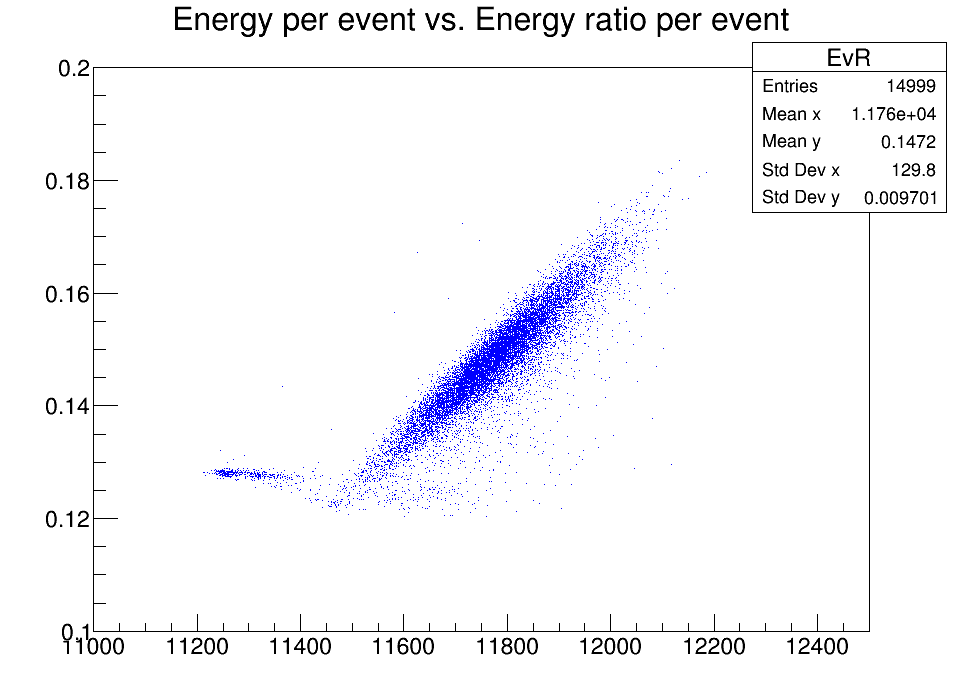
\includegraphics[width=0.65\textwidth]{../Pictures/12709-EvR.png}
	\caption{Plot of $E$ against $R$ for the secondary hadron beam with $n = 10$ (Run 12709).}
	\label{figure:testbeam/results/EvR}
\end{figure}

An appropriate cut can be used to select electron events. [Information about the cut]. Adding in the information from the RD52's muon trigger, muons and pions can then also be separated. Using both the cut and the muon trigger, we can thus produce spectra for each individual type of particle in the run.

[...]

The main goal of the data analysis is to characterise the response of the detector, and to measure the selection efficiencies of the detectors to various particle types. Once this is done, this will also give us a detailed account of the beam composition during each of the runs, which can be used for further work.

In order to do this, several ways to select for different particle types are necessary. The first way was using the preshower detector and muon trigger, which are both designed to discriminate between electrons and muons (respectively), with a high selection efficiency. These are used to create ``reference'' samples, [...]

The second way is to perform a kinematic selection using variables from the calorimeter. This is done using the E vs. R plot (normalised for beam energy) to select a region corresponding to a certain particle type. For example, the plot below shows this plot for Run [xxx] (X GeV hadrons) with the regions corresponding to hadrons and electrons highlighted. These regions overlap, meaning that attempting to select for hadrons using an ellipse around that region will also result in a non-insignificant number of electrons also being selected.

In order to perform a pure selection using the calorimeter, an extremely tight cut was used, focusing on the red spot at the centre of the hadron region. This ensures that the majority of events that pass the cut are hadrons, giving a high-purity selection. The purity of this selection can be assessed by using the appropriate preshower or muon trigger, excluding all non-hadron particles, and comparing the two numbers. If $N_{K}$ is the number of particles passing the selection with only the kinematic cut, and $N_{K+T}$ is the number of particles passing \emph{both} the kinematic cut and the triggers, then the selection efficiency for hadrons $\epsilon_{hadron}$ is given by:

\begin{displaymath}
	\epsilon_{hadron} = \frac{N_{K+T}}{N_{K}}
\end{displaymath}

This was then done with the same process for electrons and muons, to obtain the individual selection efficiencies. % Should probably go through the process with the actual cut values itself.

% Results of this selection, and the matrix?